\title{Computer Vision}
\author{
        Assignment 1 - Pixel Operations\\
Spring 2023
}
\date{}
\documentclass[12pt]{article}
\usepackage[margin=0.7in]{geometry}
\usepackage{graphicx}
\usepackage{float}
\usepackage{amsmath}
\usepackage{tikz}
\usetikzlibrary{calc}
\usepackage{graphicx}

\begin{document}
\maketitle


\section*{Introduction}
In this first assignment we want to get you comfortable with importing and exporting images as well applying basic point-processing algorithms.   \\

\noindent
\textbf{Subsequent assignments will likely be far more involved, but we want to you getting your “hands dirty” as soon as possible!}\\

\noindent
In this assignment, as with all of our assignments, you shouldn't be using built-in functions that violate the ``spirit'' of the assignment.  For instance, in part 3, you can't use a function like \emph{rgb2gray}, for part 5 you can't use any functions that do gamma correction for you, in part 6 you \textbf{cannot}t use a function like \emph{rgb2hsv} or \emph{hsv2rgb} and in part 7 you \textbf{cannot} use the \emph{hist} function.\\

\noindent
In this assignment you will demonstrate your ability to:
\begin{itemize}
\item Obtain images and import them into Matlab
\item Demonstrate the application of several pixel-processing algorithms.
\item Render histograms and images
\end{itemize}

\section*{Grading}
\begin{table}[h]
\begin{centering}
\begin{tabular}{|l|l|}
\hline
Theory Questions & 15pts \\
RGB $\rightarrow$ Grayscale & 15pts\\
RGB $\rightarrow$ Binary & 15pts\\
Gamma Correction & 20pts\\
Changing Hue & 15pts\\
Histograms & 20pts\\
\hline
\textbf{TOTAL} & 100pts\\
\hline
\end{tabular}
\caption{Grading Rubric}
\end{centering}
\end{table}

\newpage
\section{(15pts) Theory Questions}
\begin{enumerate}
\item (5pts) Given a pixel in RGB color space with the values $R=100, B=10, G=200$, what is the value of this pixel in HSV color space?  Should your computations.\\
Ans: \begin{align*}
R &= \frac{100}{255} = 0.392 \\
B &= \frac{10}{255} = 0.039 \\
G &= \frac{200}{255} = 0.784 \\
V &= \max(R,G,B) = \max(0.392,0.039,0.784) = 0.784 \\
\Delta &= \max(R,G,B) - \min(R,G,B) = \max(0.392,0.039,0.784) - \min(0.392,0.039,0.784) \\
\Delta &= 0.784 - 0.039 = 0.745 \\
S &= \frac{\Delta}{V} = \frac{0.745}{0.784} \approx 0.950 \\
H &= 120° + 60° * \frac{(B - R)}{\Delta} = 120° + 60° * \frac{(0.039 - 0.392)}{0.745} \approx 193°
\end{align*}

Since max(R,G,B) is G. Therefore, the value of this pixel in HSV color space is (193°,95\%,78\%).\\

\item 	Based on observing a histogram perhaps we decided to create the following pixel intensity mappings in order to stretch the values of a particularly compressed area (you may assume the full range is [0,255]):\\

\begin{center}
[0,10]$\rightarrow$[0,100]\\
(10,200]$\rightarrow$(100,150]\\
(200,255]$\rightarrow$(150,255]
\end{center}

\begin{enumerate}
\item(2pts) Draw a 2D graph showing these mappings.  The x-axis will be the input values and the y-axis will be the output values.\\
Ans: \\
\begin{figure}[htp]
    \centering
    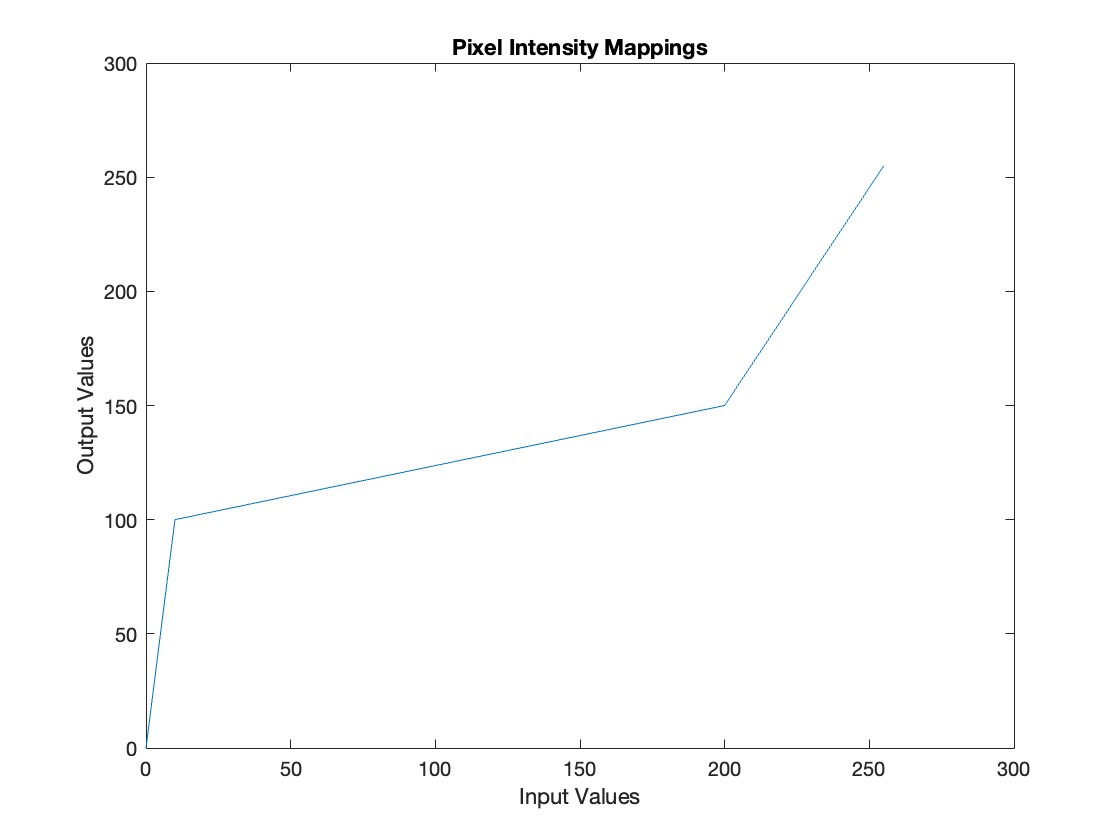
\includegraphics[width=7cm]{mappings.jpg}
\end{figure}

\item (4pts) What are the equations for these mappings?\\
Ans: For each of these mappings, we can calculate the slope of the linear function that maps the input values to the output values. The slopes are calculated as follows:

For the first mapping [0, 10] → [0, 100], the slope is (100 - 0) / (10 - 0) = 10.\\
For the second mapping (10, 200] → (100, 150], the slope is (150 - 100) / (200 - 10) = 0.263.\\
For the third mapping (200, 255] → (150, 255], the slope is (255 - 150) / (255 - 200) = 2.1.\\

Using these slopes, we can write the equations for each of the three regions of the piecewise-linear function as follows:

For input values in the range [0, 10], the output value is calculated as\\ output = 10 * input.\\
For input values in the range (10, 200], the output value is calculated as\\ output = 0.263 * (input - 10) + 100.\\
For input values in the range (200, 255], the output value is calculated as\\ output = 2.1 * (input - 200) + 150.\\

\item (1pt) Given a value of 50, what will this value be mapped to?\\
Ans: Since 50 falls in the range (10, 200], we should use the equation for that region to calculate the output value. \\
The equation for this region is output = 0.263 * (input - 10) + 100.

Substituting the input value of 50 into this equation, we get: \\
output = 0.263 * (50 - 10) + 100 = 0.263 * 40 + 100 = 110.52

Therefore, an input value of 50 will be mapped to an output value of approximately 110.52 using the piecewise-linear function defined by the pixel intensity mapping.\\

\item (3pts) In your own words, describe the effect of this mapping.\\
Ans: This mapping stretches the values of a particularly compressed area in the image. The pixel intensity mappings you provided specify that pixel values in the range [0, 10] should be mapped to the range [0, 100], pixel values in the range [10, 200] should be mapped to the range [100, 150], and pixel values in the range [200, 255] should be mapped to the range [150, 255].

This mapping will have the effect of increasing the contrast in the region between pixel values 0 and 10 by stretching those values over a wider range in the output image. Similarly, it will compress the contrast in the region between pixel values 10 and 200 by mapping those values to a narrower range in the output image. Finally, it will increase the contrast in the region between pixel values 200 and 255 by stretching those values over a wider range in the output image.

Overall, this mapping will enhance the contrast of the image by stretching and compressing specific regions of pixel values.


\end{enumerate}
\end{enumerate}


\newpage
\section{Dataset}
For the programming component of this assignment, you may use a \emph{color} image of your choosing.  Make sure that you include your image with your submission so that we can recreate your results.  In each of the following sections you'll be asked to output images.  The images will also be included in your report.

\begin{figure}[htp]
    \centering
    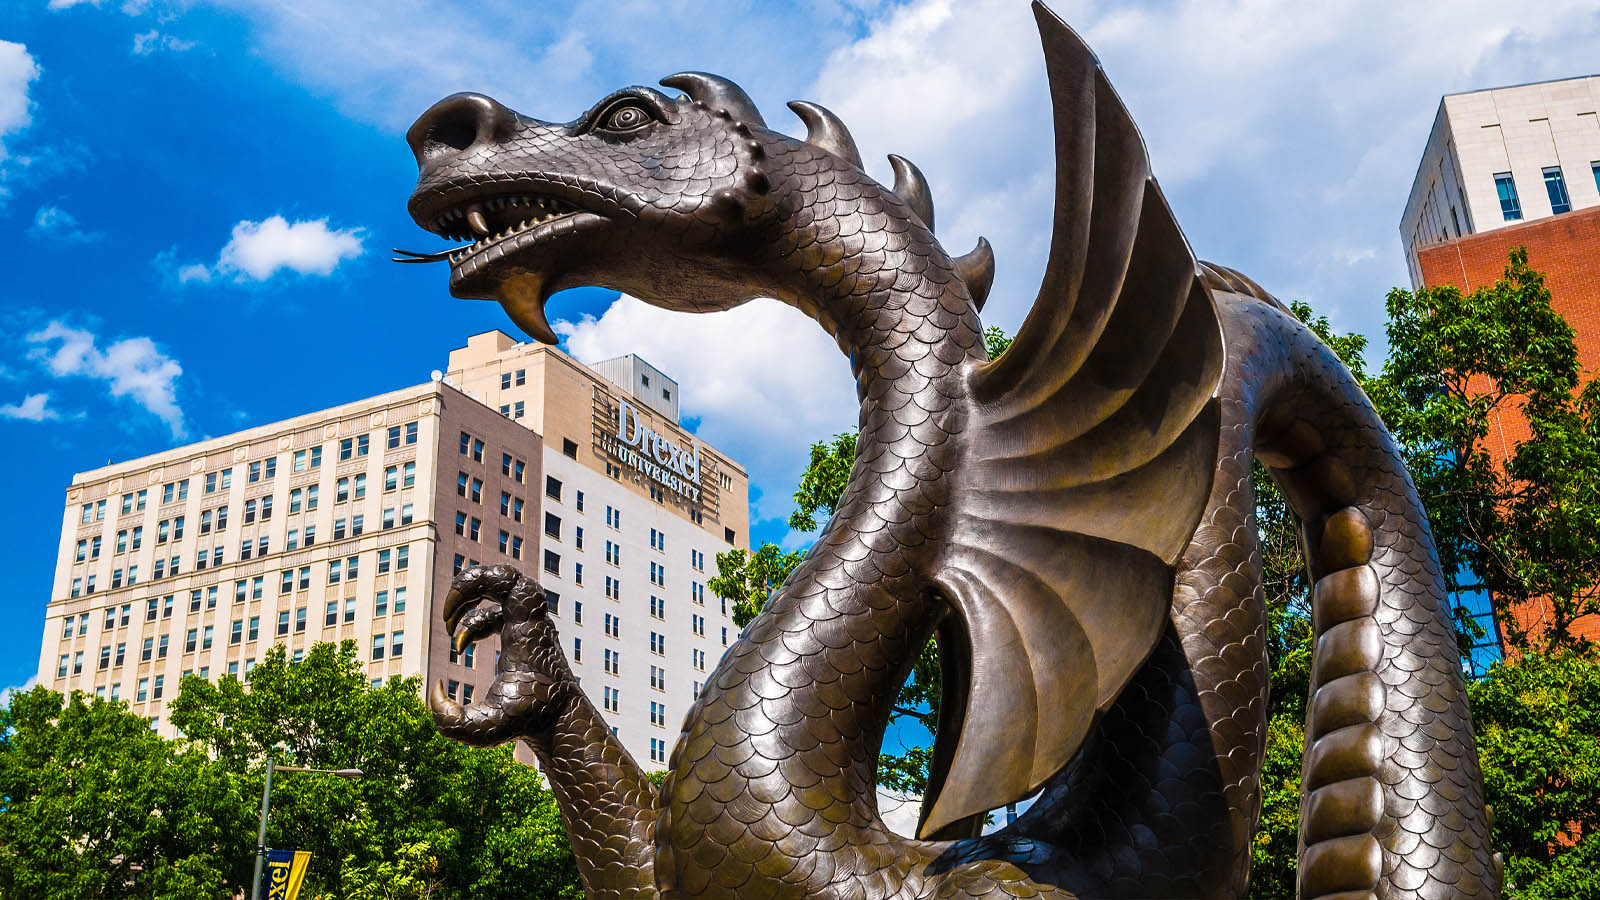
\includegraphics[width=8cm]{input_1.jpg}
\end{figure}

\section{(15pts) RGB $\rightarrow$ Grayscale}
\noindent
The first point-processing thing we want to be able to do is to convert an image from color to grayscale.\\

\noindent
Read in your color image and use the following formula to convert it to a grayscale image.  You \textbf{may not} use a built-in function to do this (i.e rgb2gray).\\

\begin{equation}
Gray=0.2989R+0.5870*G+0.1140B
\end{equation}

\begin{figure}[htp]
    \centering
    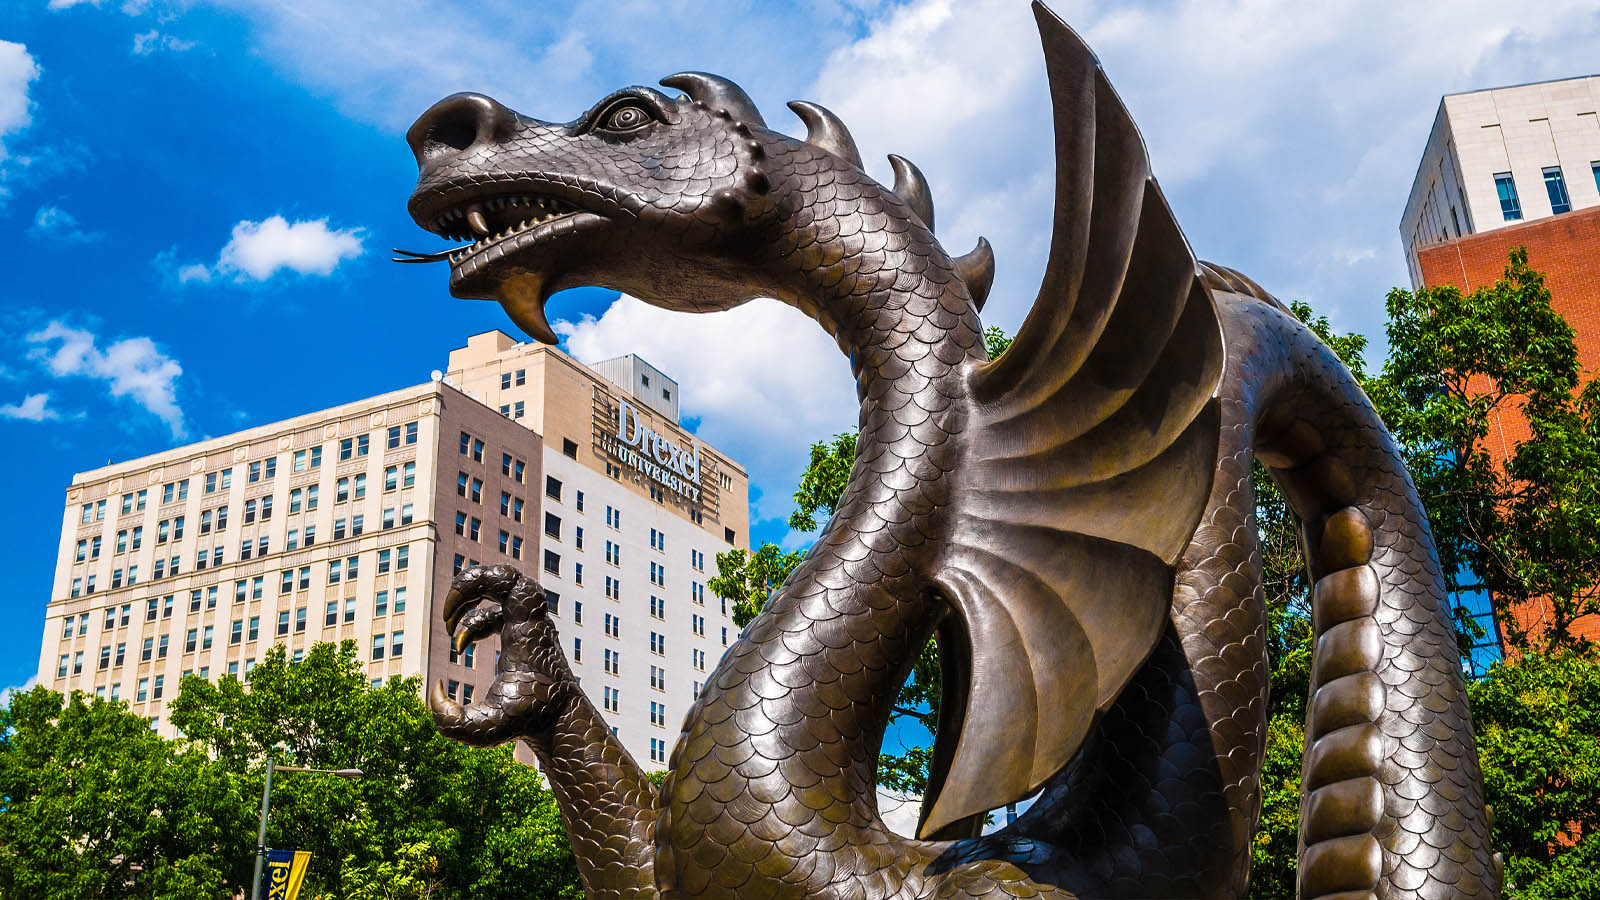
\includegraphics[width=8cm]{input_1.jpg}
    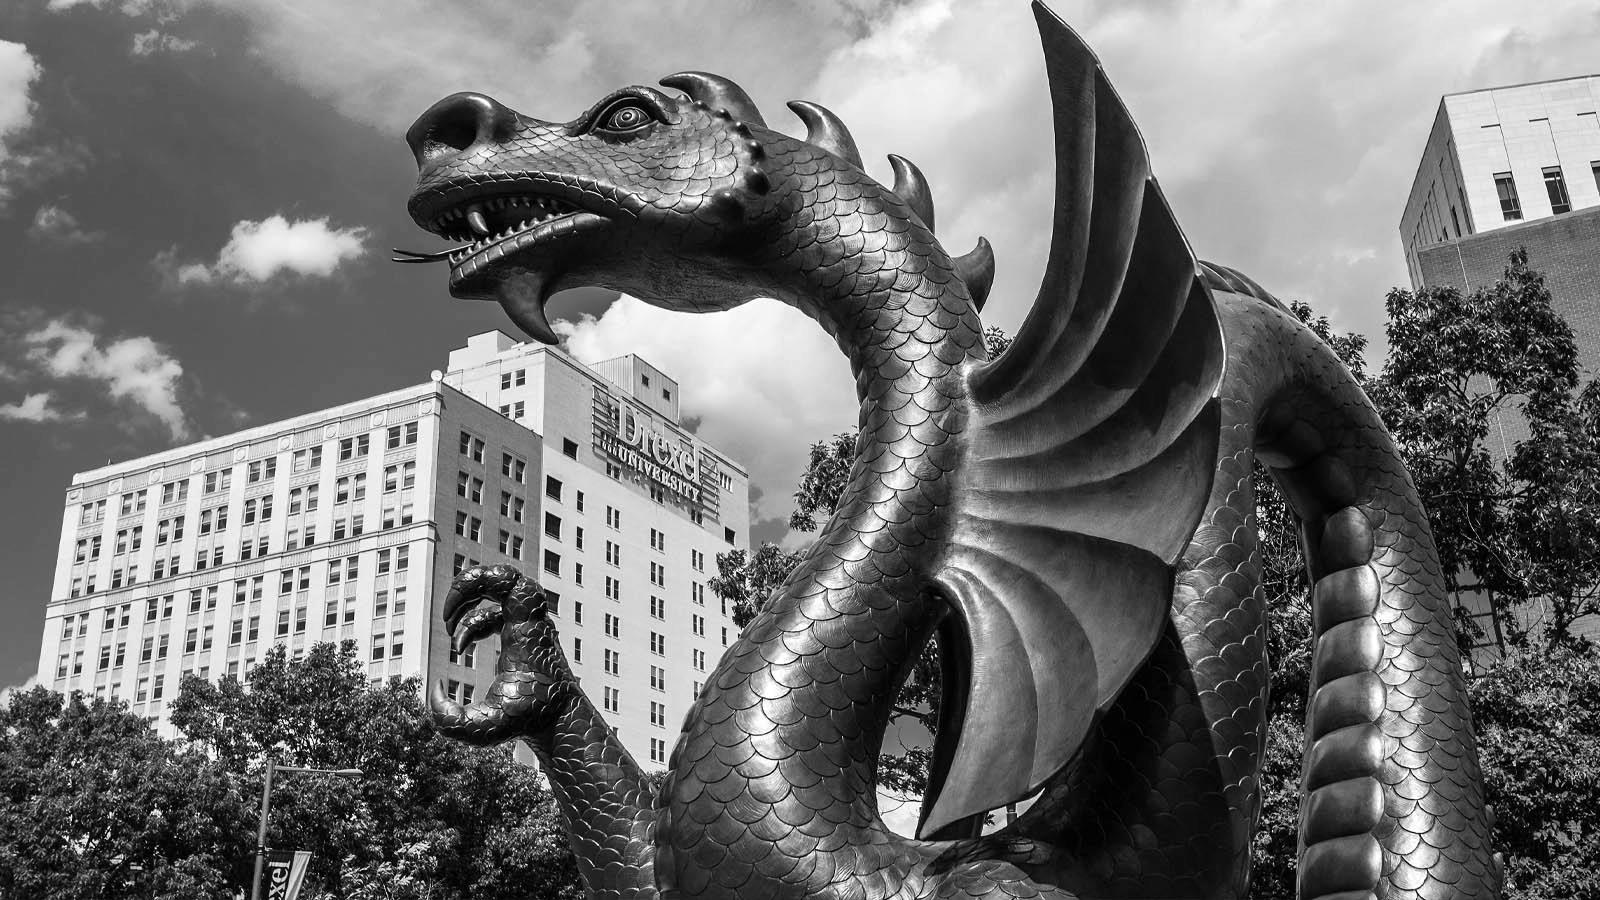
\includegraphics[width=8cm]{grayscale.jpg}
\end{figure}

\newpage
\section{(15pts) RGB $\rightarrow$ Binary}
In this part, we want to be able to convert your color image into a binary image, where each pixel is either black or white.\\

\noindent
To do this, first convert your image to grayscale (using what you did in the previous part), then produce three binary images, one for each of the following thresholds (as percentages of maximum possible intensity value):
\begin{itemize}
\item t=25\%
\item t=50\%
\item t=75\%
\end{itemize}

\begin{figure}[htp]
    \centering
    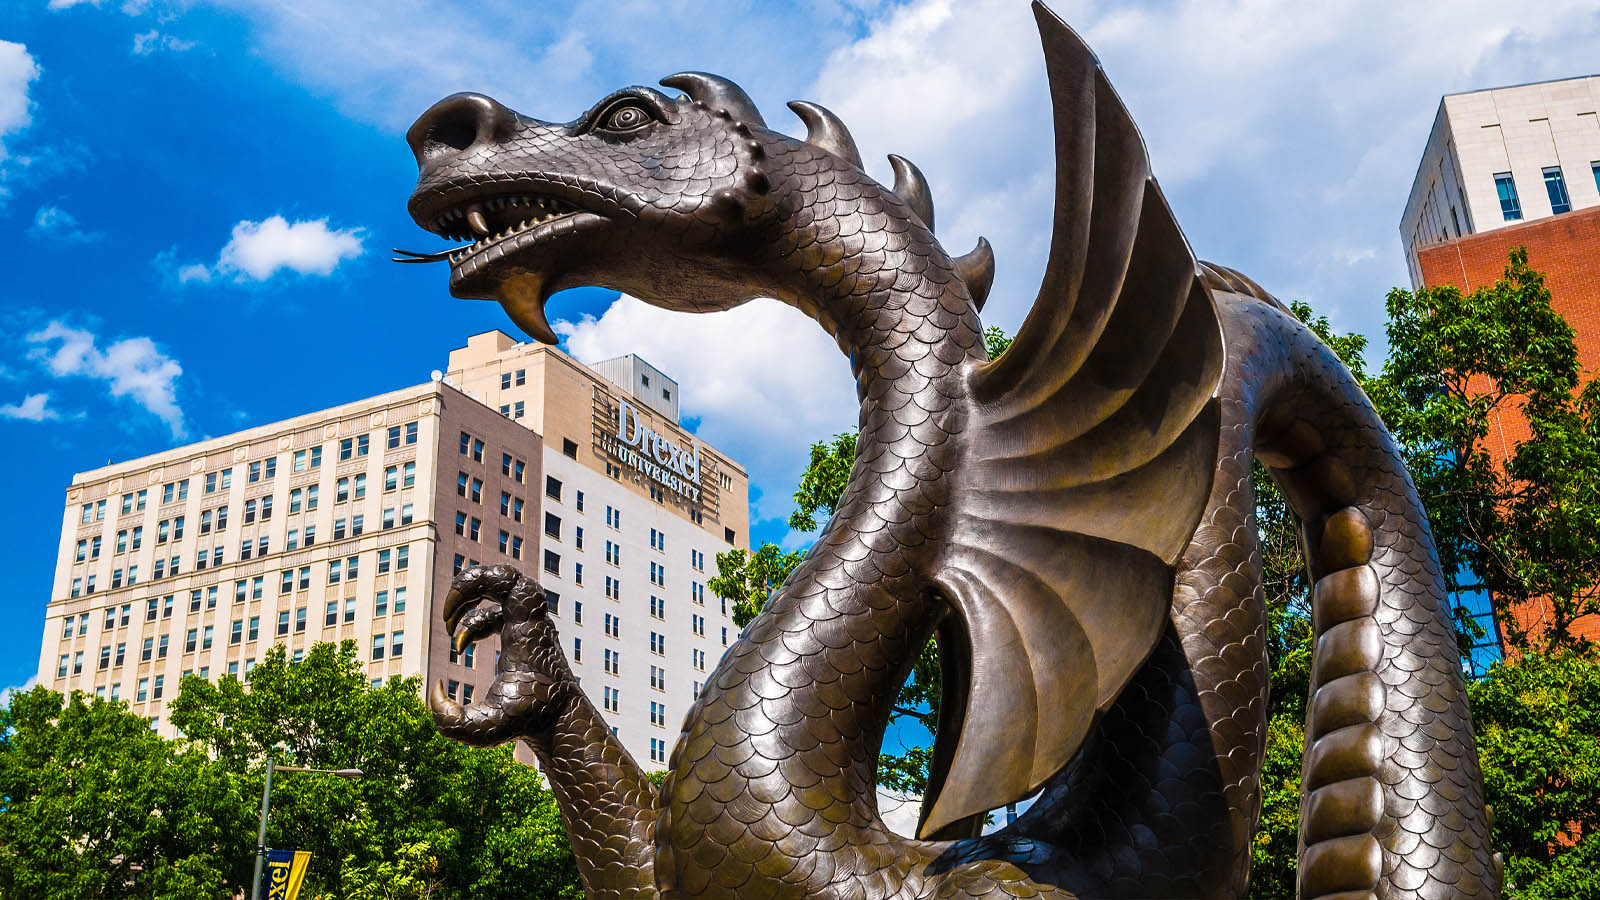
\includegraphics[width=8cm]{input_1.jpg}
    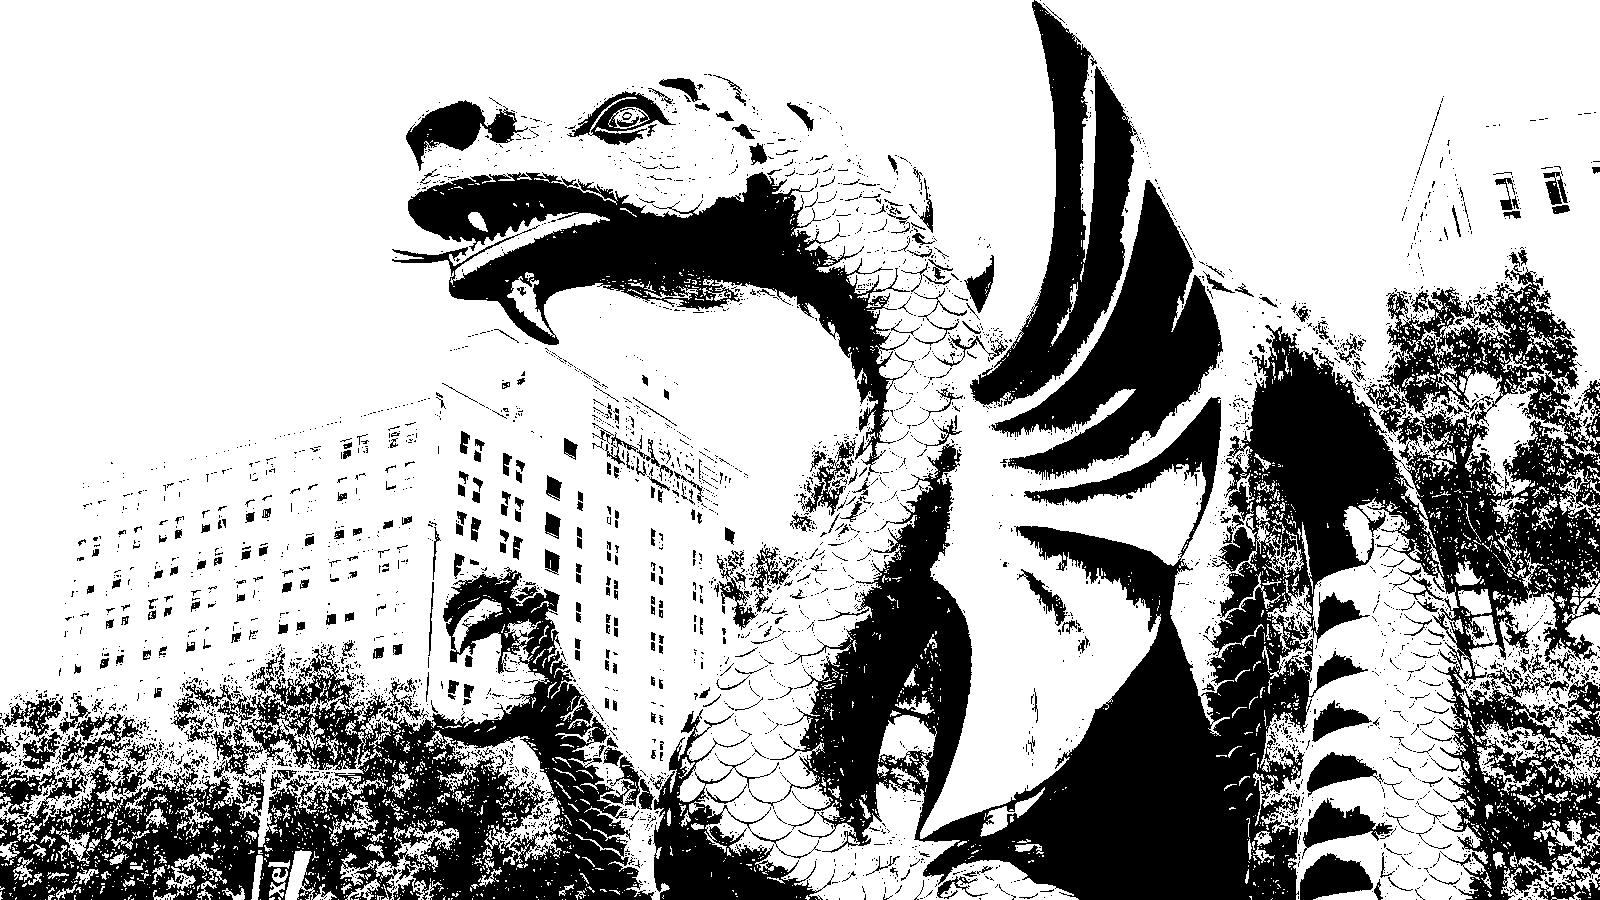
\includegraphics[width=8cm]{binary_25_t.jpg}
    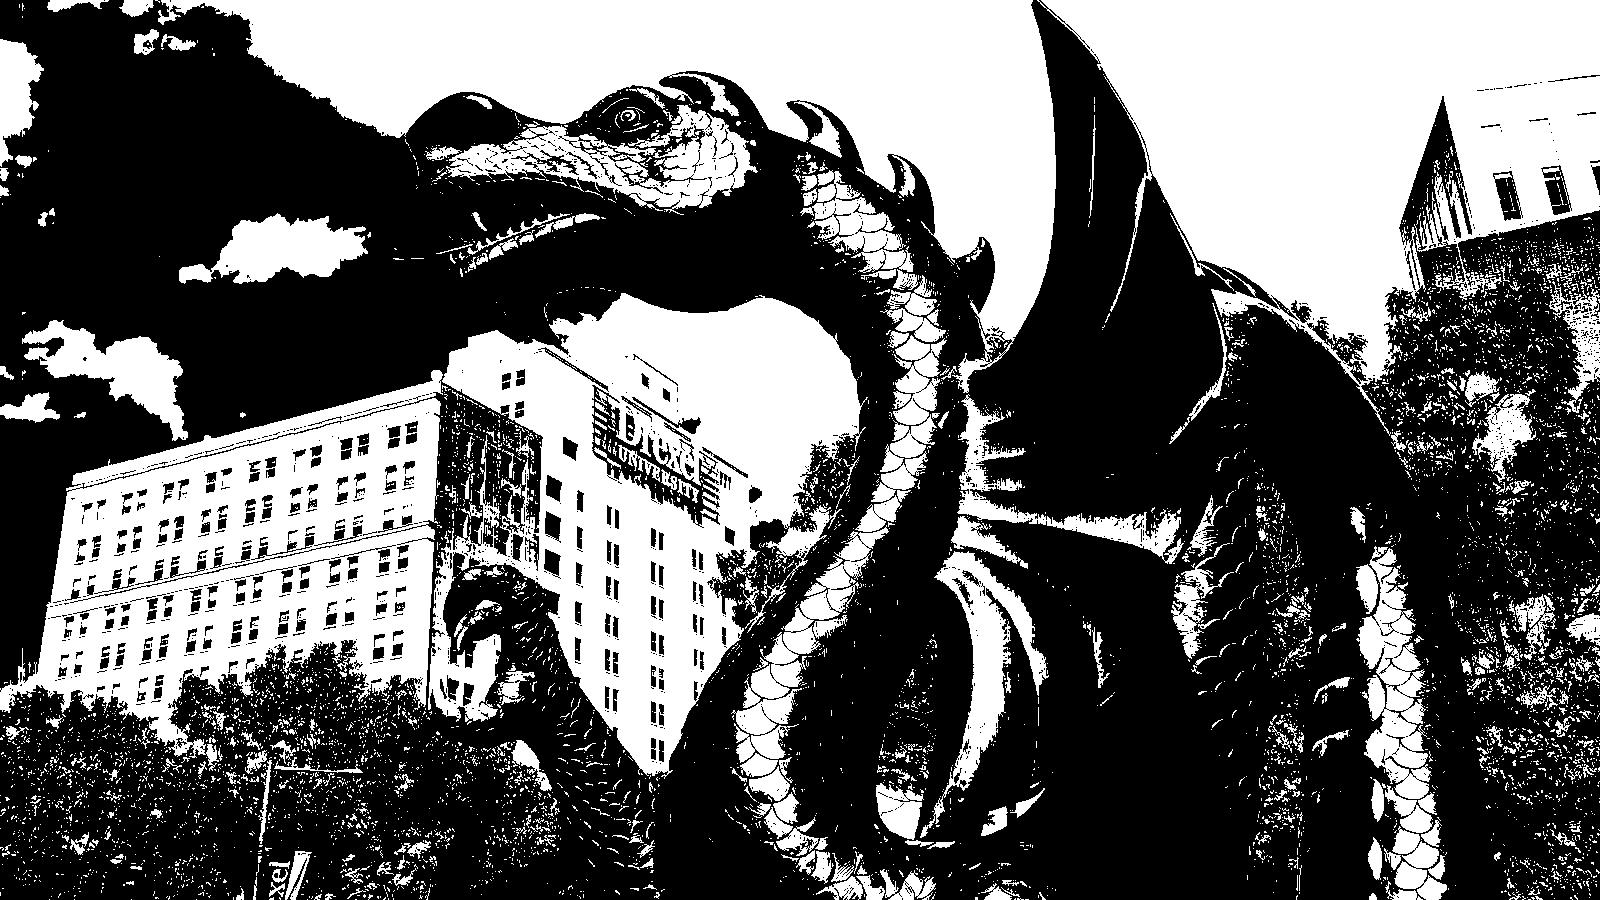
\includegraphics[width=8cm]{binary_50_t.jpg}
    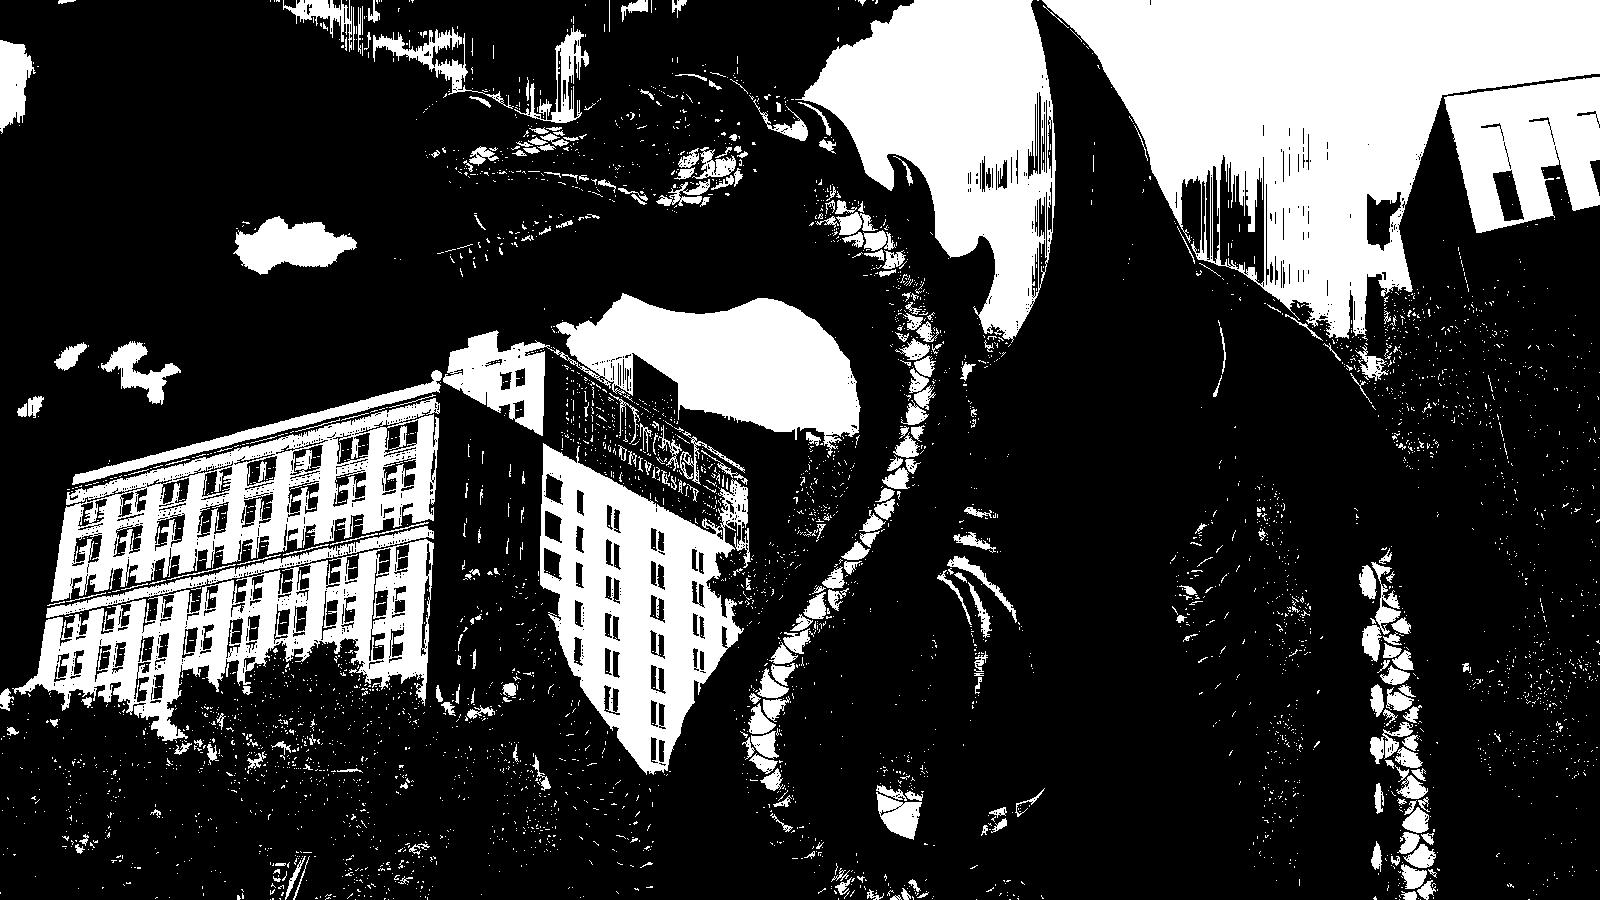
\includegraphics[width=8cm]{binary_75_t.jpg}
\end{figure}

\newpage
\section{(20pts) Gamma Correction}
In this part, we want to apply some gamma correction to your image.  Making sure that your RGB values are in the range $[0,1]$, apply gamma correction to each channel (independently) via the formula $s=r^\gamma$ (we'll let $c=1$).  Do this for each of the following values of gamma (producing three images):

\begin{itemize}
\item $\gamma=0.2$
\item $\gamma=1$
\item $\gamma=50$
\end{itemize}

\begin{figure}[htp]
    \centering
    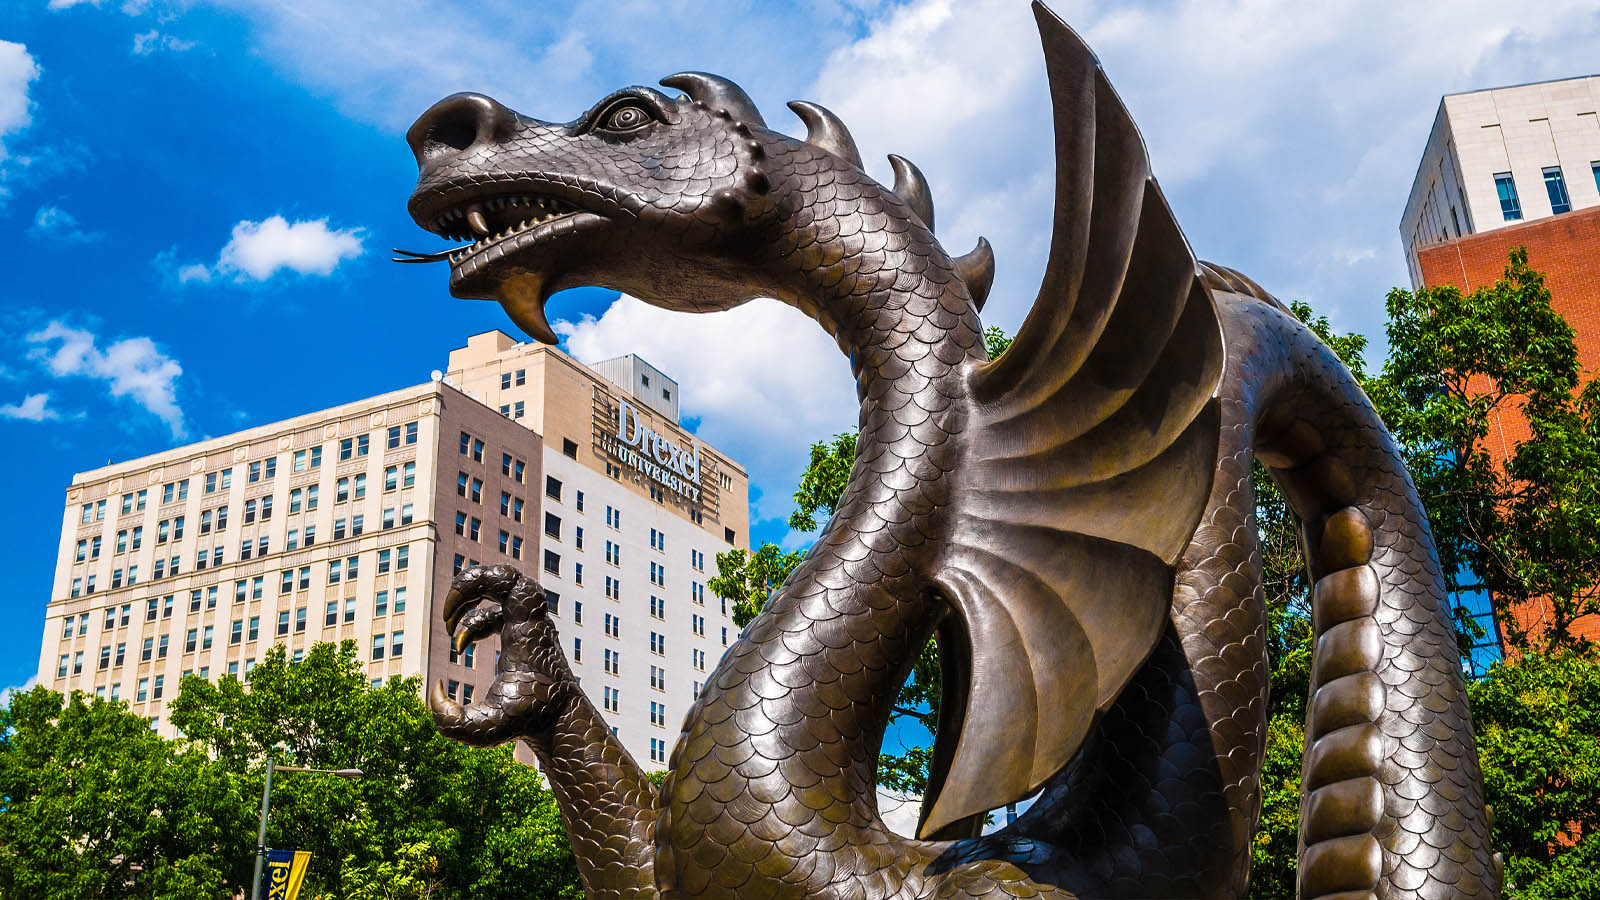
\includegraphics[width=8cm]{input_1.jpg}
    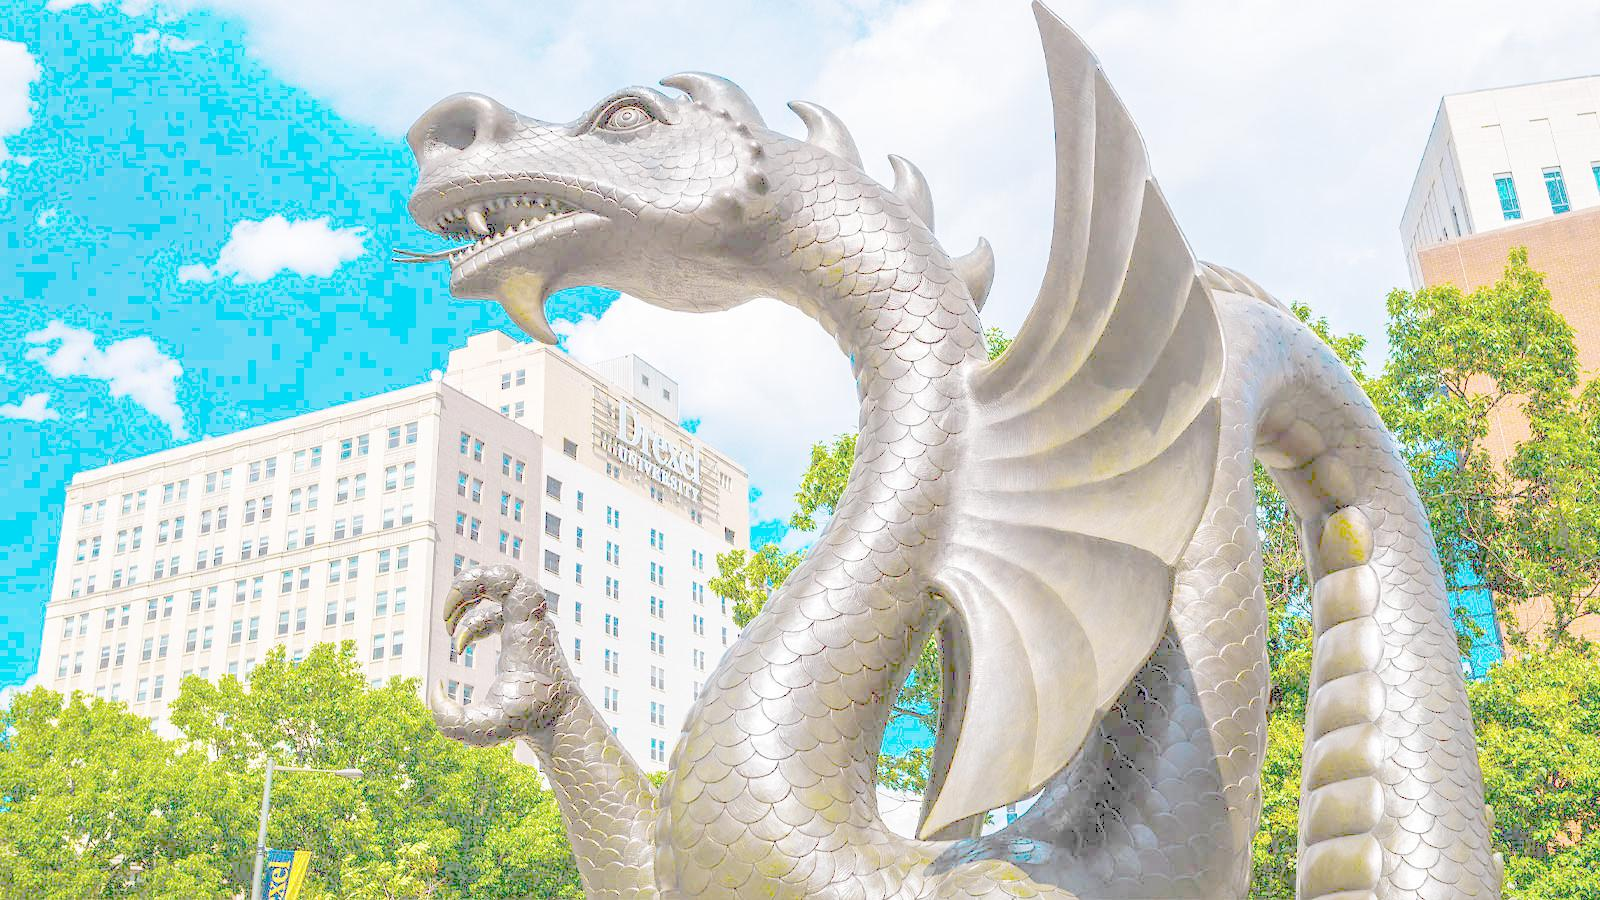
\includegraphics[width=8cm]{gamma_0.2.jpg}
    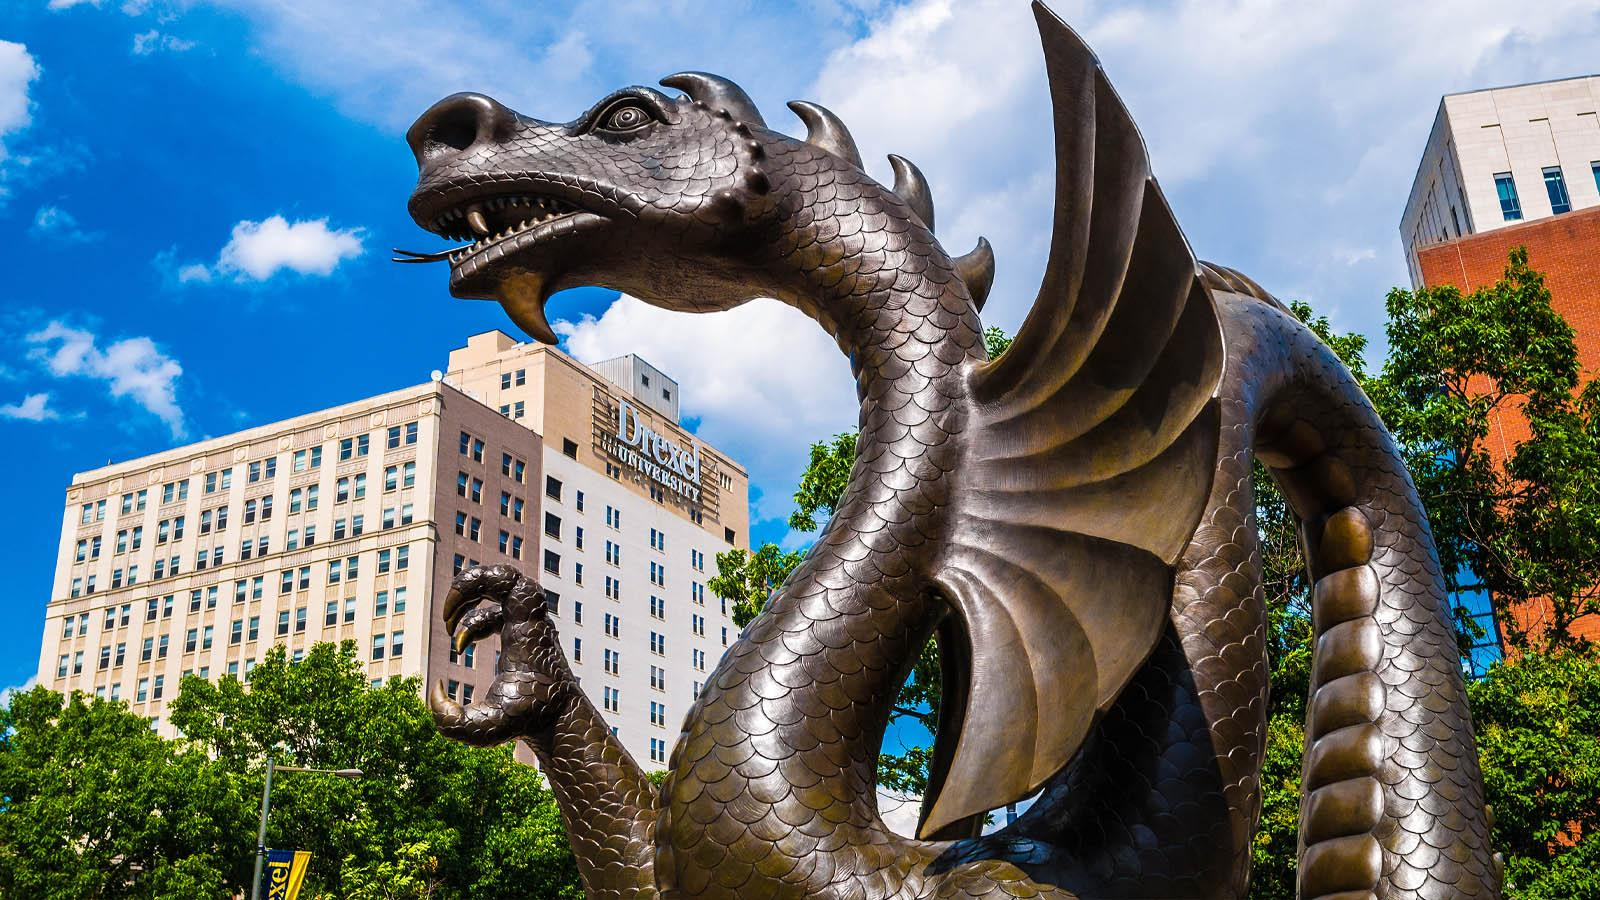
\includegraphics[width=8cm]{gamma_1.jpg}
    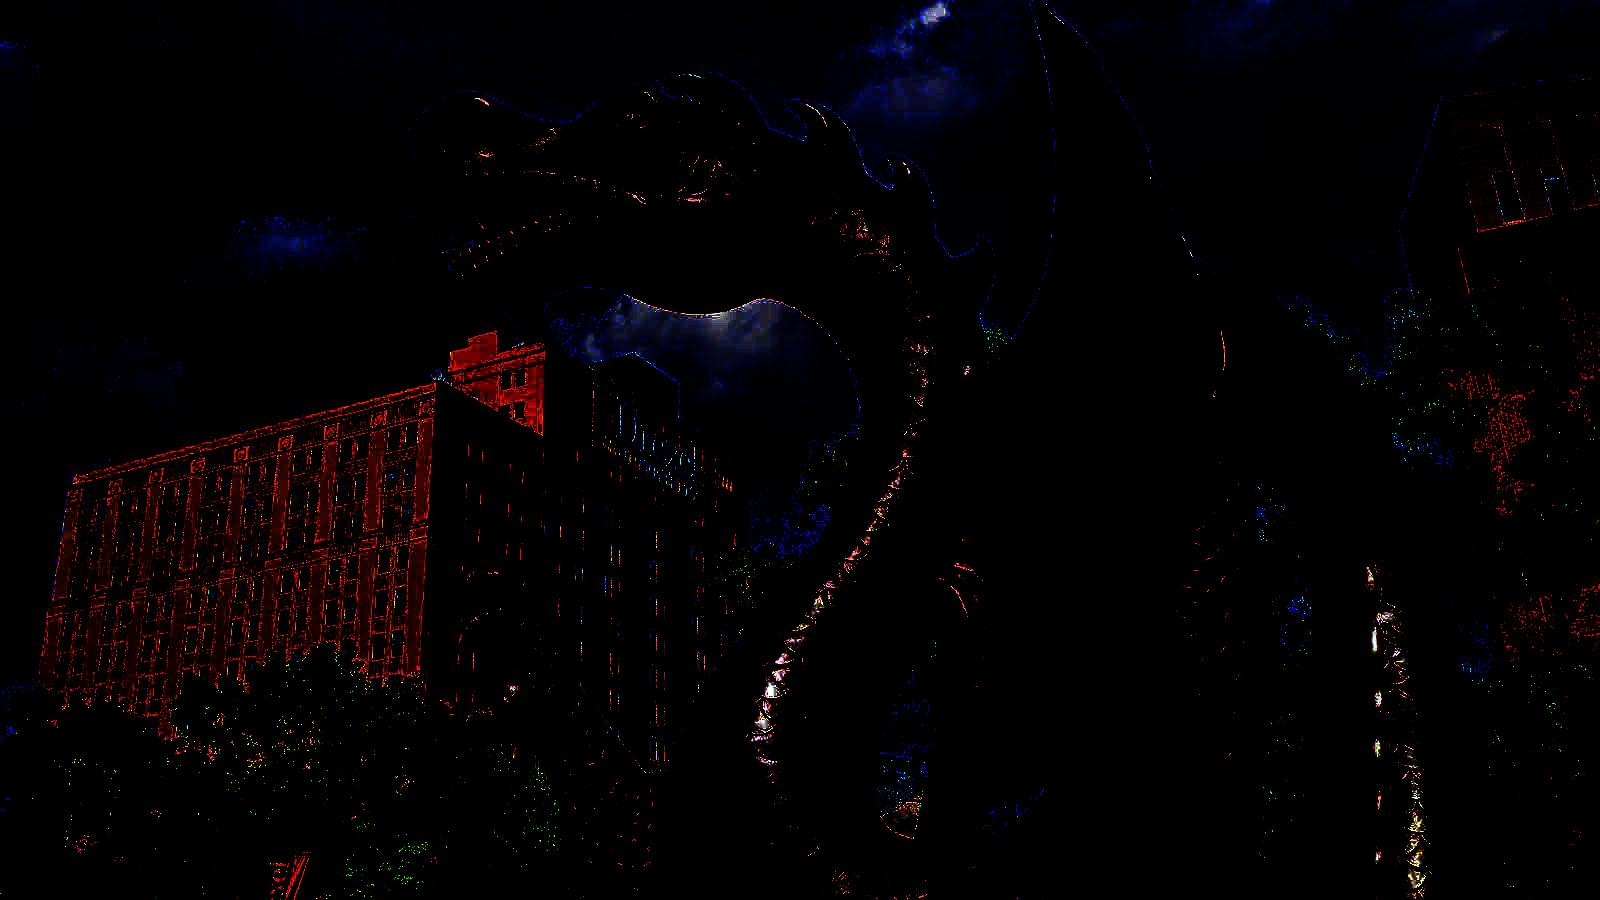
\includegraphics[width=8cm]{gamma_50.jpg}
\end{figure}

\newpage
\section{(15pts) Changing Hue}
In this part we'll go from RGB space to HSV space, change the hue, then return to RGB space.\\

\noindent
Create a new RGB image that has the hue value of pixels increased by a value of $50^\circ$.  Do this by first converting your image from RGB to HSV, increasing the hue, then returning to RGB space.  Keep in mind that when you increase the hue values, you might end up with values out of the range $[0,360]$.   Think about how to deal with this in your implementation.  You \textbf{cannot} use functions that due the color space conversion for you (like \emph{rgb2hsv}).

\begin{figure}[htp]
    \centering
    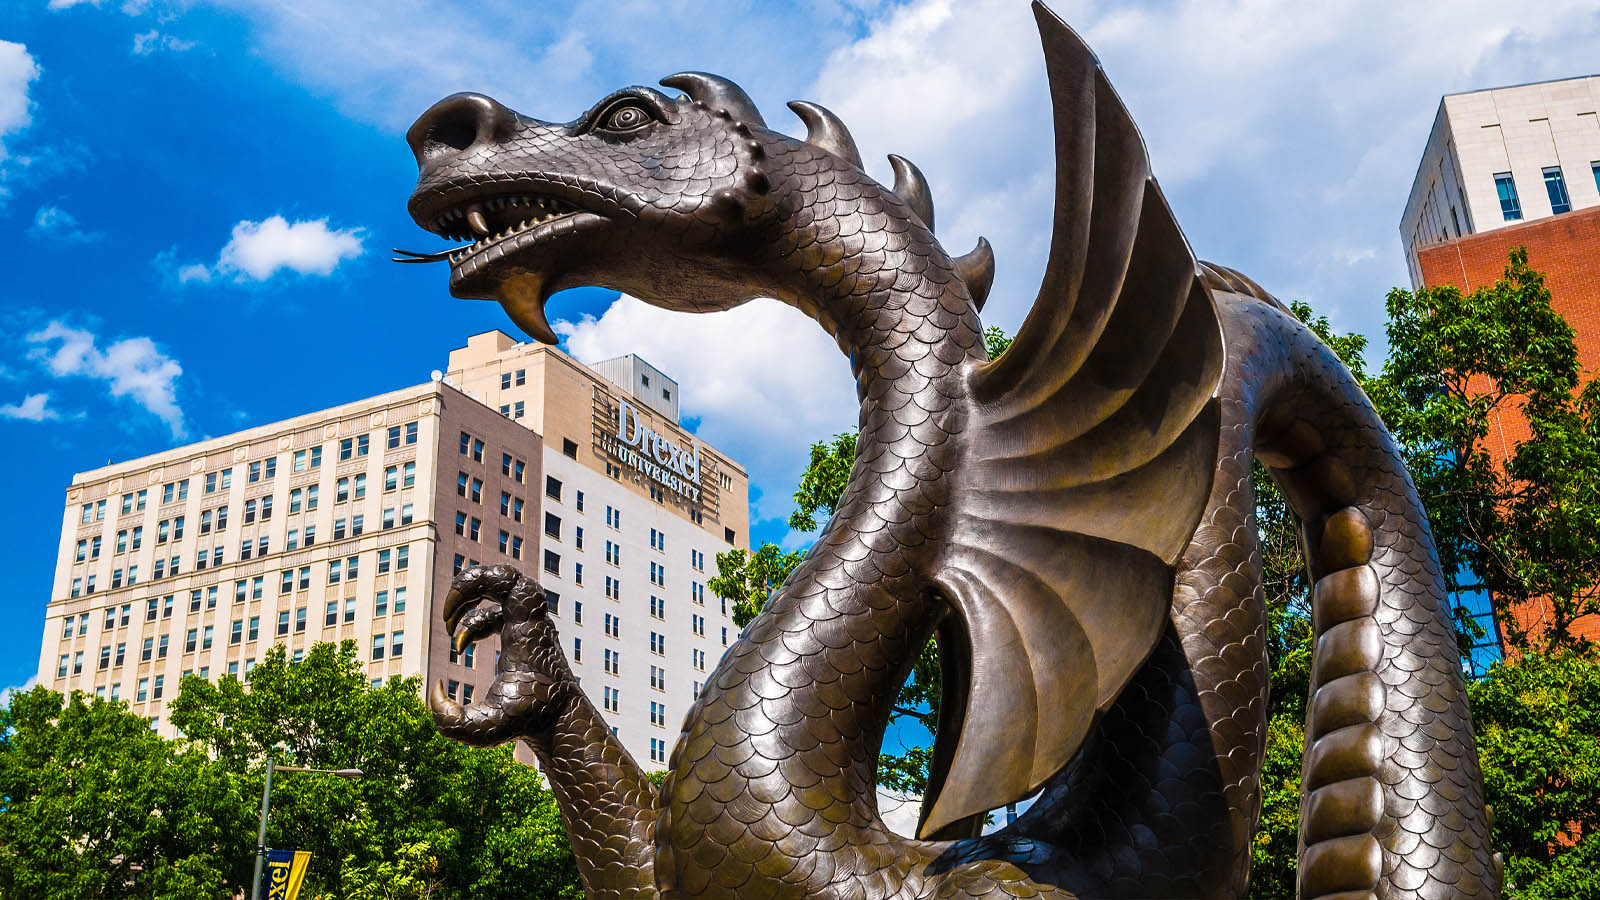
\includegraphics[width=14cm]{input_1.jpg}
    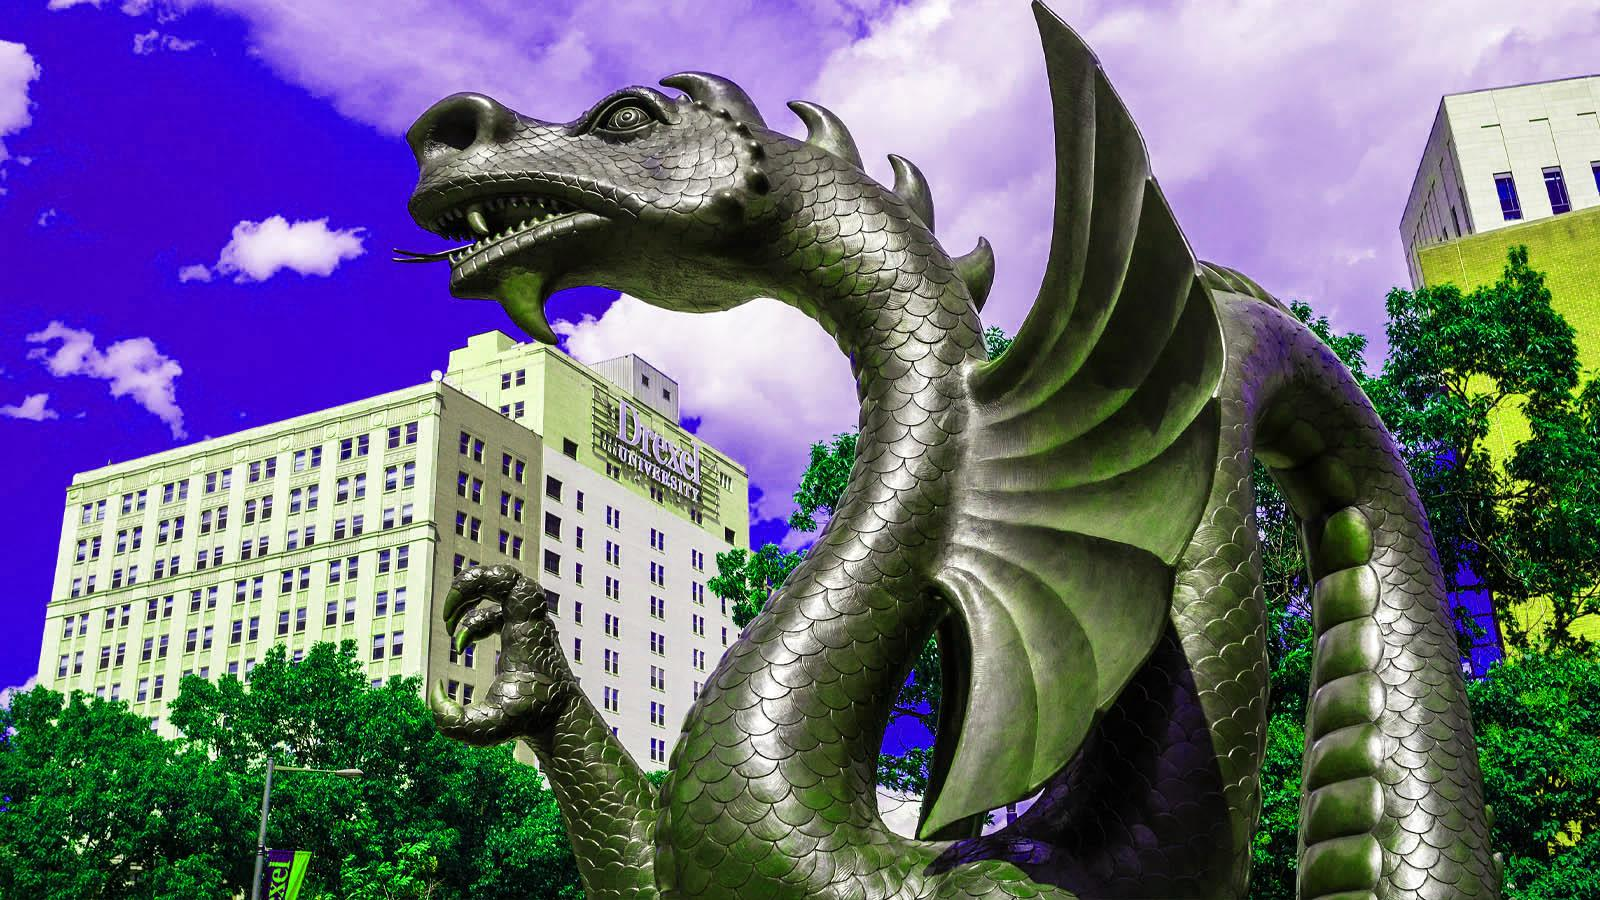
\includegraphics[width=14cm]{hue_image.jpg}
\end{figure}

\newpage
\section{(20 points) Histograms}
Histograms are a critical analysis tool use for many computer vision problems.  Display four histograms for your image, each of which have 256 bins.  \textbf{You may not use a built-in function to obtain the histogram}.  To plot your histogram, use the \emph{bar} function of Matlab.

\begin{itemize}
\item Grayscale histogram
\item Histogram of the red channel
\item Histogram of the green channel
\item Histogram of the blue channel.
\end{itemize}

\begin{figure}[htp]
    \centering
    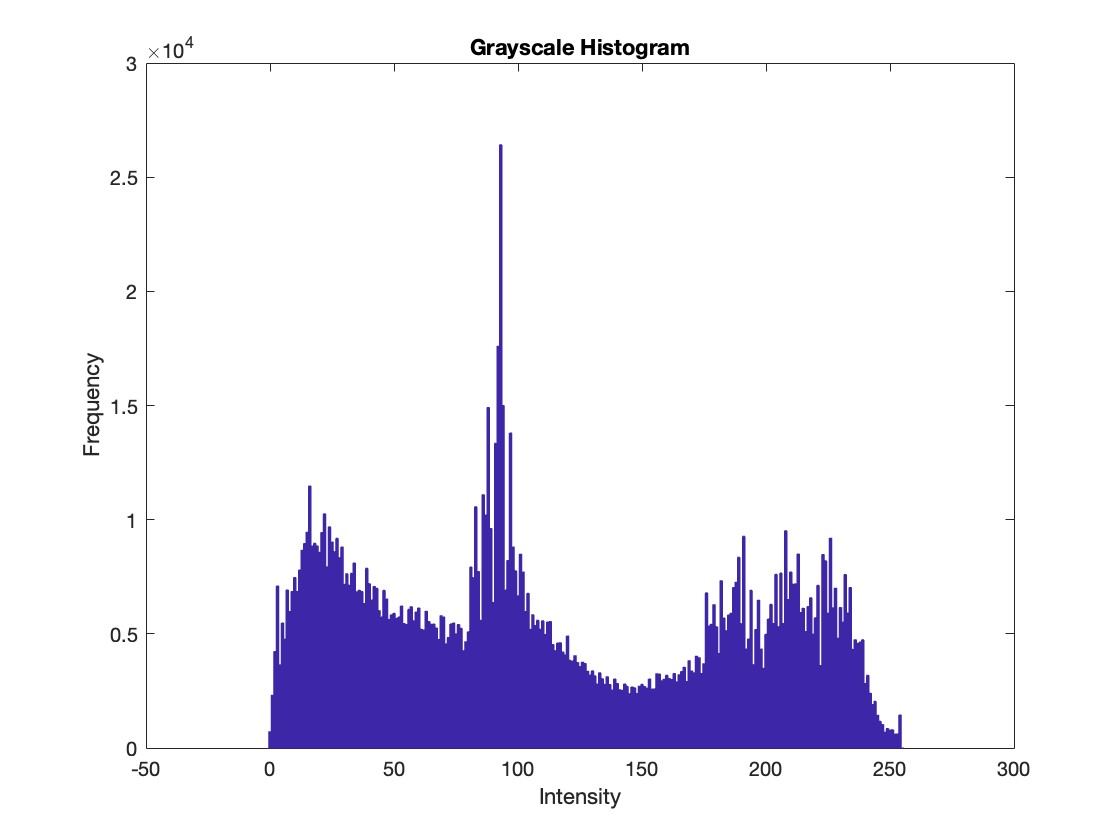
\includegraphics[width=8cm]{grayscale histogram.jpg}
    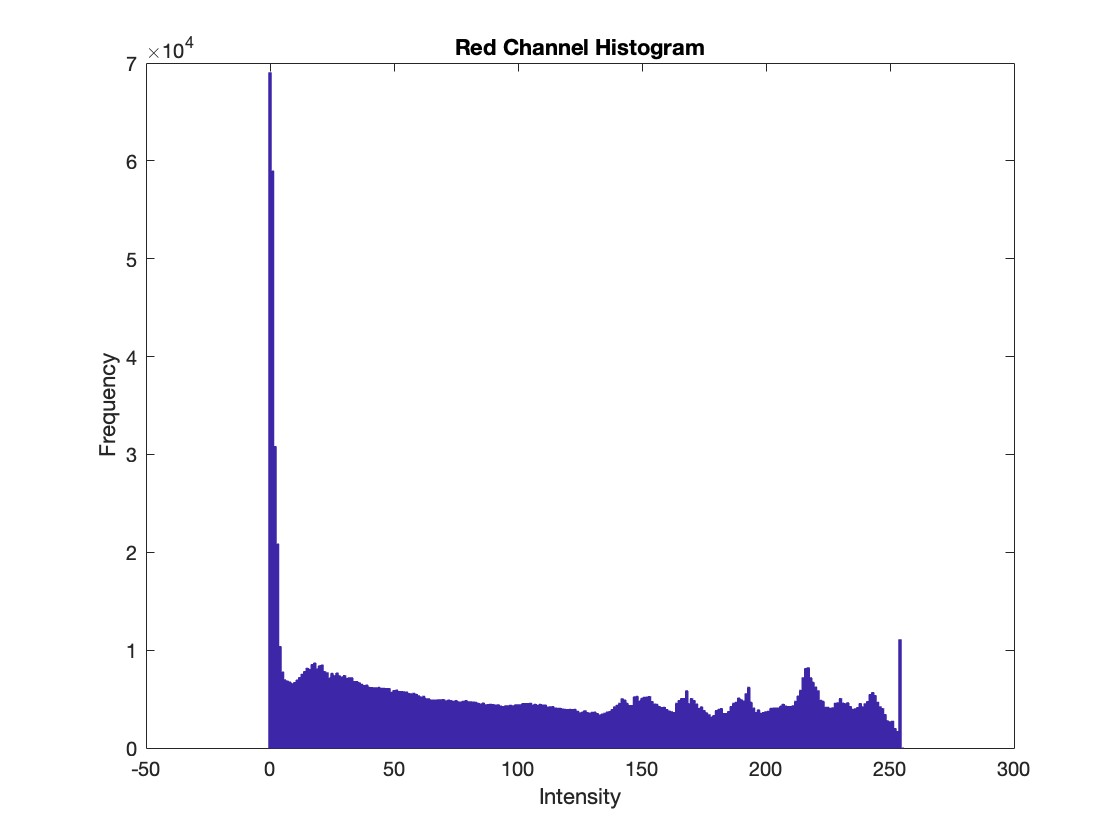
\includegraphics[width=8cm]{Red_Channel_Histogram.jpg}
    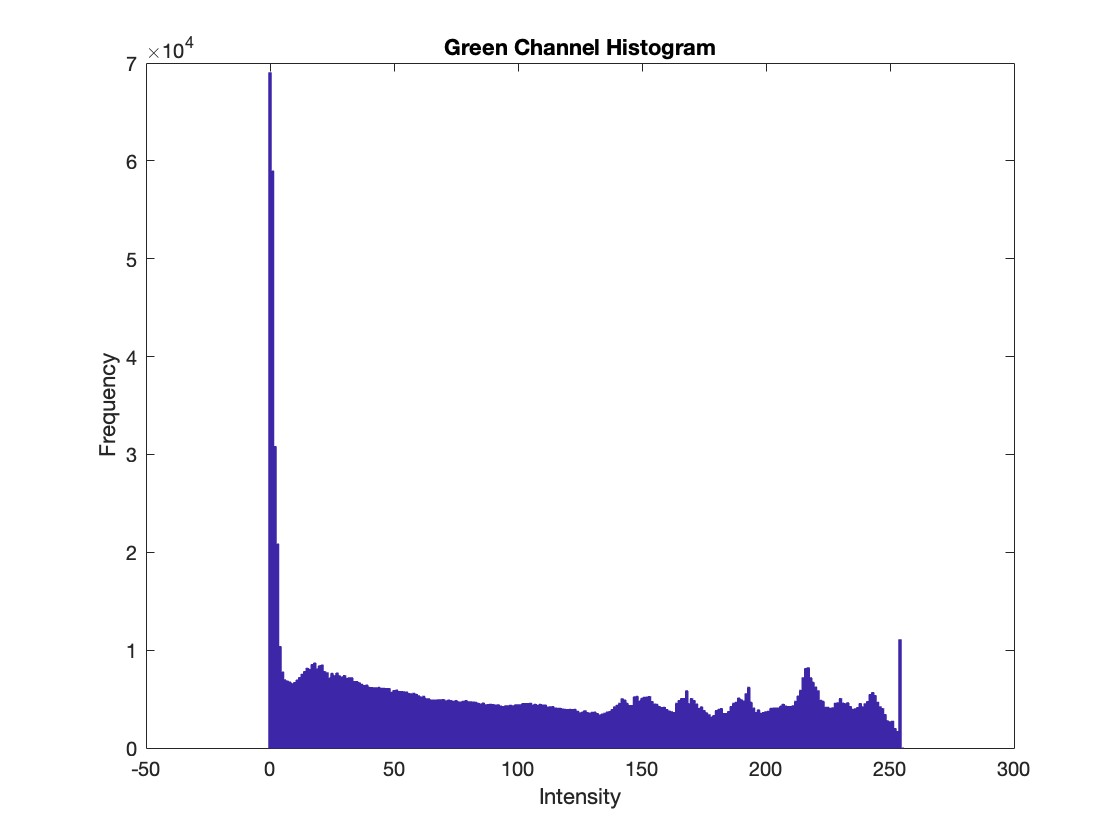
\includegraphics[width=8cm]{Green_Channel_Histogram.jpg}
    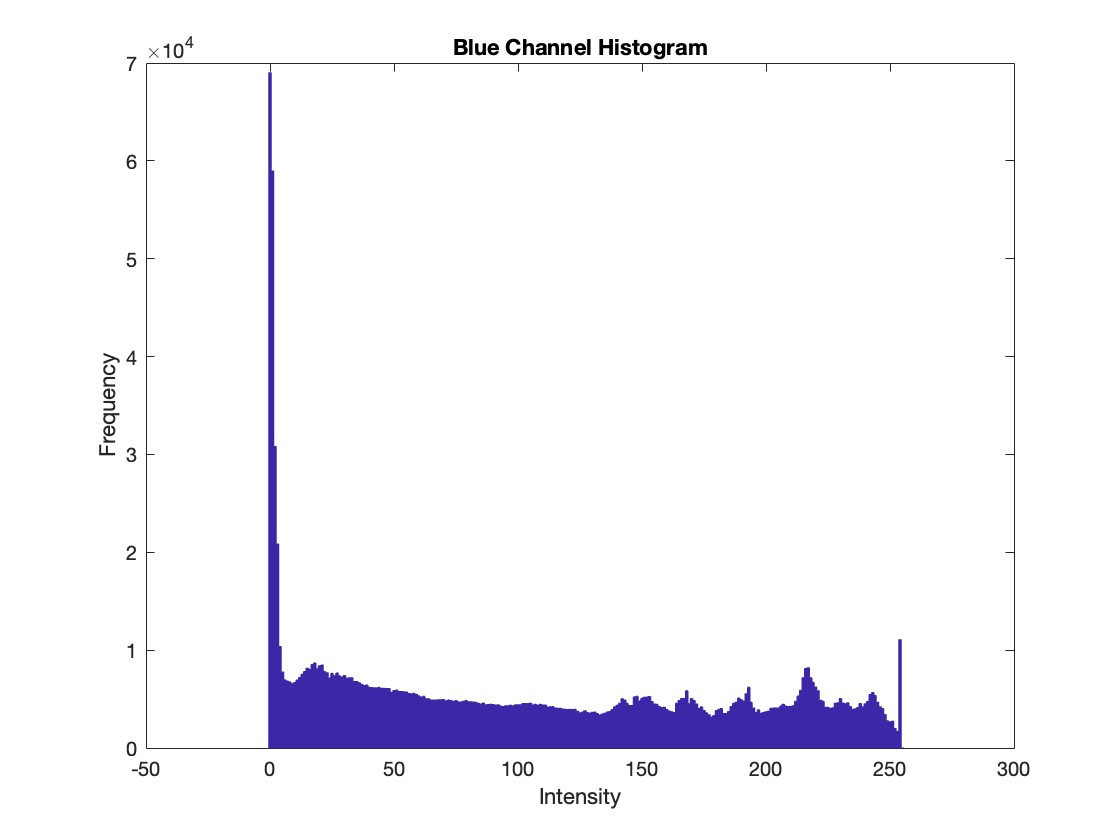
\includegraphics[width=8cm]{Blue_Channel_Histogram.jpg}
\end{figure}

\newpage
\section*{Submission}
For your submission, upload to Blackboard a single zip file containing:

\begin{enumerate}
\item PDF writeup that includes:
\begin{enumerate}
\item Your answer to the theory question(s).
\item The RGB and Gray images for Part 3.
\item The RGB and Binary images for Part 4 (so 4 images total).
\item The RGB and Gamma Corrected images for Part 5 (so 4 images total).
\item The RGB and Hue adjusted images for Part 6.
\item The histograms for Part 7 (4 total)
\end{enumerate}
\item A README text file (\textbf{not} Word or PDF) that explains:
\begin{enumerate}
\item Any unique features of your program (if applicable).
\item Any instructions on how to run your script to reproduce your results.
\end{enumerate}
\item Your source file(s).
\item The chosen image(s) that you processed.
\end{enumerate}

\end{document}

